\chapter{Práctica 5: Caracterización de Circuitos con MOSFETS}

\section{Objetivos}
Es esta práctica se pretende caracterizar un transistor MOSFET. Para comprender el funcionamiento de este transistor, se medirá las característica I-V, se determinarán los parámetros de un MOSFET de canal N (NMOSFET) y se medirá su característica de transferencia.

\section{Fundamento Teórico}
Un transistor MOSFET (Metal Oxide Semiconductor Field Effect Transistor) es un semiconductor con tres terminales:
\begin{enumerate}
    \item Puerta ($G$ del inglés \emph{gate})
    \item Drenador ($D$ del inglés \emph{drain})
    \item Fuente ($S$ del inglés \emph{source})
\end{enumerate}
La corriente que circula entre la fuente y el drenador se controla mediante el terminal de la puerta. Además, se distinguen dos tipos: los tipo N o NMOSFET (unión NPN) y los tipos P o PMOSFET (unión PNP). En cuanto a su funcionamiento, los transistores se pueden encontrar en tres regiones distintas de funcionamiento:
\begin{enumerate}
    \item \underline{Región de Corte}
    En esta región de funcionamiento, el transistor no conduce, luego $I_d = 0\;A$. La condición necesaria para este modo es la siguiente:
    \begin{equation}\begin{split}
        Corte & \Longleftrightarrow V_{GS} < V_T \\
        & I_d = 0\;A
    \end{split}\end{equation}
    donde $V_T$ representa la tensión umbral y es característica de cada transistor.
    
    \item \underline{Región Lineal}
    En esta región de funcionamiento, el transistor sí conduce. Las ecuaciones que describen este modo son:
    \begin{equation}\begin{split}
        Lineal & \Longleftrightarrow \left\{ 
            \begin{array}{l}
                 V_{GS} \geq V_T  \\
                 V_{DS} < (V_{GS} - V_T)
            \end{array}
        \right. \\
        & I_d = \frac{k}{2} \left[ 2(V_{GS} - V_T)V_{DS} - V_{DS}^2 \right]
    \end{split}\end{equation}
    donde $k$ es la transconductancia del transistor, característica del mismo.
    
    \item \underline{Región de Saturación}
    En esta región de funcionamiento, el transistor sí conduce. Las ecuaciones que describen este modo son:
    \begin{equation}\label{Ec:Sat}
    \begin{split}
        Saturaci\Acute{o}n & \Longleftrightarrow \left\{ 
            \begin{array}{l}
                 V_{GS} \geq V_T  \\
                 V_{DS} \geq (V_{GS} - V_T)
            \end{array}
        \right. \\
        & I_d = \frac{k}{2} \;(V_{GS} - V_T)^2
    \end{split}\end{equation}
    
\end{enumerate}

Para ver la característica de transferencia de un transistor NMOSFET, se va a trabajar con el circuito de la figura \ref{fig:Circuito_CarTrans} con la entrada en $V_i$ y salida en $V_0\;(=V_{DS})$. Este circuito es el de un \textbf{inversor}, ya que para potenciales de entrada altos, el potencial de salida será bajo y vicerversa. La ecuación de $V_0$ es:
\begin{enumerate}
    \item \underline{Corte} ($V_i < V_T$)
    $$V_0 = V_{DD}$$
    \item \underline{Saturación} ($V_i > V_T$)
    $$V_0 = V_{DD} - \frac{k\;R_D}{2}\;(V_i - V_T)^2$$
    \item \underline{Lineal} ($V_i \gg V_T$)
    $$V_0 = \frac{1+kR_D(V_i-V_T)}{kR_D} - \frac{\sqrt{(1+kR_D(V_i-C_T))^2-2kR_DV_{DD}}}{kR_D}$$
\end{enumerate}

Además, sean $V_i^*$ y $V_0^*$ los valores de transición de saturación a lineal.
\begin{equation}\label{Ec:SatALin_CarTrans}
    V_i^* = V_0^* + V_T = \frac{-1+\sqrt{1+2kR_DV_{DD}}}{kR_D} + V_T
\end{equation}

Por tanto, según la teoría respecto al circuito \ref{fig:Circuito_CarTrans},
\begin{equation}\label{Ec:CarTrans}
    V_0(V_i) = \left\{
    \begin{array}{lcc}
         V_{DD} & si & V_i < V_T \\
         V_{DD} - \frac{k\;R_D}{2}\;(V_i - V_T)^2 & si & V_T \leq V_i \leq V_i^*\\
         \frac{1+kR_D(V_i-V_T)}{kR_D} - \frac{\sqrt{(1+kR_D(V_i-V_T))^2-2kR_DV_{DD}}}{kR_D} & si & V_i^* < V_i
    \end{array}
    \right.
\end{equation}  


\begin{figure}
    \centering
    \begin{circuitikz}
    \ctikzset{tripoles/mos style/arrows}
        \draw (0,0) to [american resistor, l=$R_G$] (2, 0);
        \draw (3,-0.77) to [short] (3, -1);
        \draw (3, 3) to [short, *-] (3,2.5)
        to [american resistor, l=$R_D$] (3, 0.77);
        \draw (3, 0.77) to [short] (3.5,0.77);

        \draw (0,0) node [left] {$V_i$}
        (3,3) node [above] {$V_{DD}$}
        (3.5, 0.77) node [right] {$V_0$}
        (3, -1) node [ground] {}
        (3,0) node [nmos] {};
    \end{circuitikz}
    \caption{Montaje Experimental para la medida de la característica de transferencia de un NMOSFET}
    \label{fig:Circuito_CarTrans}
\end{figure}

\newpage
Para ver la característica I-V de un transistor NMOSFET en saturación, se va a trabajar con el circuito de la figura \ref{fig:Circuito_I-V}. Este se encuentra en saturación al tener la puerta y drenador cortocircuitados. El potencial medido es $V_0$ $(=V_{DS}=V_{GS})$.

\begin{figure}
    \centering
    \begin{circuitikz}
    \ctikzset{tripoles/mos style/arrows}
        \draw (3, 0.77) to [short] (1.5,0.77)
        to [short] (1.5,0)
        to [short] (2,0);
        
        \draw (3,-0.77) to [short] (3, -1);
        \draw (3, 3) to [short, *-] (3,2.5)
        to [american resistor, l=$R_D$] (3, 0.77);
        \draw (3, 0.77) to [short] (3.5,0.77);

        \draw (3,3) node [above] {$V_{DD}$}
        (3.5, 0.77) node [right] {$V_0$}
        (3, -1) node [ground] {}
        (3,0) node [nmos] {};
    \end{circuitikz}
    \caption{Montaje Experimental para la medida de la característica I-V de un NMOSFET}
    \label{fig:Circuito_I-V}
\end{figure}


\section{Material}
\begin{itemize}
    \item \underline{Fuente de alimentación:} fuente de tensión de corriente continua empleada para proporcionarle tensión al circuito. El modelo empleado es FAC-363B.
    \item \underline{Polímetro digital:} dispositivo empleado para realizar diversas medidas en el circuito. Es usado principalmente en corriente continua para medir la resistencia, diferencia de potencial o capacidad de un condensador, por ejemplo.
    \item \underline{Resistencias}
    \item \underline{Circuito integrado 4007} este circuito integrado contiene 6 transistores MOSFET, tres de canal N y tres de canal P. Como se ve en la figura \ref{fig:Circuito4007}, los tres de abajo son los de tipo N, por lo que se usará uno de ellos.
    \begin{figure}
        \centering
        \begin{subfigure}[b]{0.3\textwidth}
             \centering
             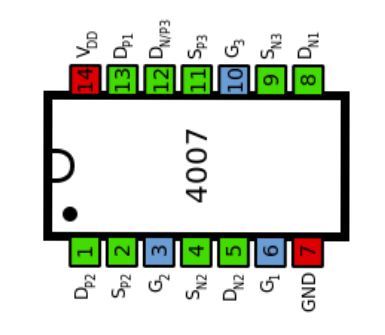
\includegraphics[width=\textwidth]{Imágenes 05/Pinout_4007.png}
         \end{subfigure}
         \hfill
         \begin{subfigure}[b]{0.3\textwidth}
             \centering
             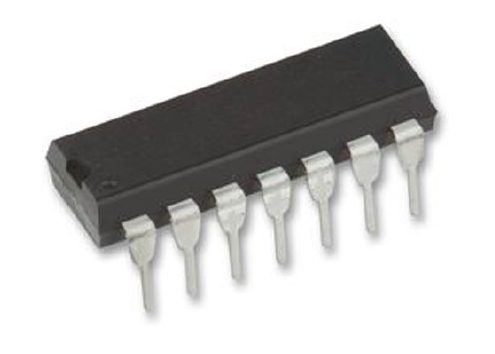
\includegraphics[width=\textwidth]{Imágenes 05/Img_4007.png}
         \end{subfigure}
         \hfill
         \begin{subfigure}[b]{0.3\textwidth}
             \centering
             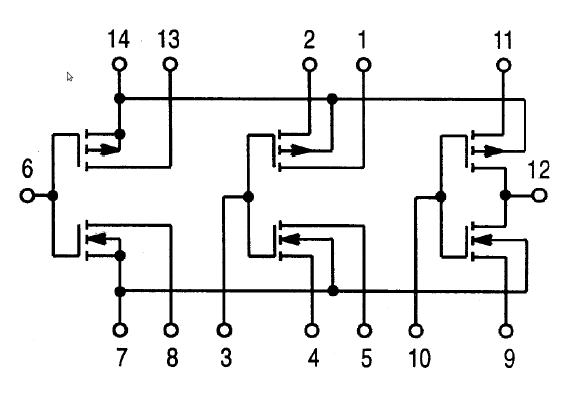
\includegraphics[width=\textwidth]{Imágenes 05/Schematics_4007.png}
         \end{subfigure}
         \hfill
        \caption{Circuito integrado 4007}
        \label{fig:Circuito4007}
    \end{figure}
    
    \item \underline{Protoboard}
\end{itemize}


\section{Desarrollo y resultados}

\subsection{Característica de Transferencia}
Se ha montado el circuito de la figura \ref{fig:Circuito_CarTrans}, donde los valores de los elementos empleados en él son:
\begin{itemize}
    \item $R_D = 0.998\;k\Omega$
    \item $R_G = 0.99\;M\Omega$
    \item $V_{DD} \approx 15\;V$
\end{itemize}
Una vez medidas estas, se han medido diversas magnitudes conforme se variaba el valor de $V_i$, el potencial de entrada. Los datos obtenidos se muestran en la figura \ref{fig:Datos_CarTrans}, donde cada columna representa:
\begin{description}
    \item [Columna 1:] Potencial de entrada teórico ($V_i^{teo}$) [$V$]. Dado por la fuente de alimentación.
    \item [Columna 2:] Potencial de entrada real ($V_i^{exp}$) [$V$]. Medido con el polímetro.
    \item [Columna 3:] Caída de potencial en entre la puerta y la fuente del transistor ($V_{GS}$) [$V$]. Medido con el polímetro.
    \item [Columna 4:] Caída de potencial en entre el drenador y la fuente del transistor ($V_{DS}$) [$V$]. Medido con el polímetro.
    \item [Columna 5:] Caída de potencial en la resistencia de la puerta ($V_{RG}$) [$V$]. Medido con el polímetro.
    \item [Columna 6:] Caída de potencial en la resistencia del drendor ($V_{RD}$) [$V$]. Medido con el polímetro.
    \item [Columna 7:] Intensidad que circula por la puerta [$A$].\\ Calculada como $I_G = \frac{V_{RG}}{R_G}$.
    \item [Columna 8:] Intensidad que circula entre el drenador y la fuente [$A$].\\ Calculada como $I_D = \frac{V_{RD}}{R_D}$.
\end{description}

\begin{figure}
    \centering
    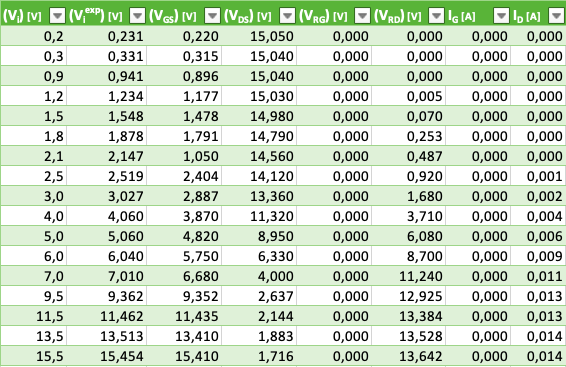
\includegraphics[width=11cm]{Imágenes 05/Tabla_Datos_CarTrans.png}
    \caption{Datos obtenidos en el circuito de la figura \ref{fig:Circuito_CarTrans}.}
    \label{fig:Datos_CarTrans}
\end{figure}

En la figura \ref{fig:CarTrans_Exp} se observa la característica de transferencia del circuito \ref{fig:Circuito_CarTrans} tomando como entrada el potencial en la puerta $V_i = V_G$, y como salida el potencial en el drenador $V_0 = V_D $.

\begin{figure}
    \centering
    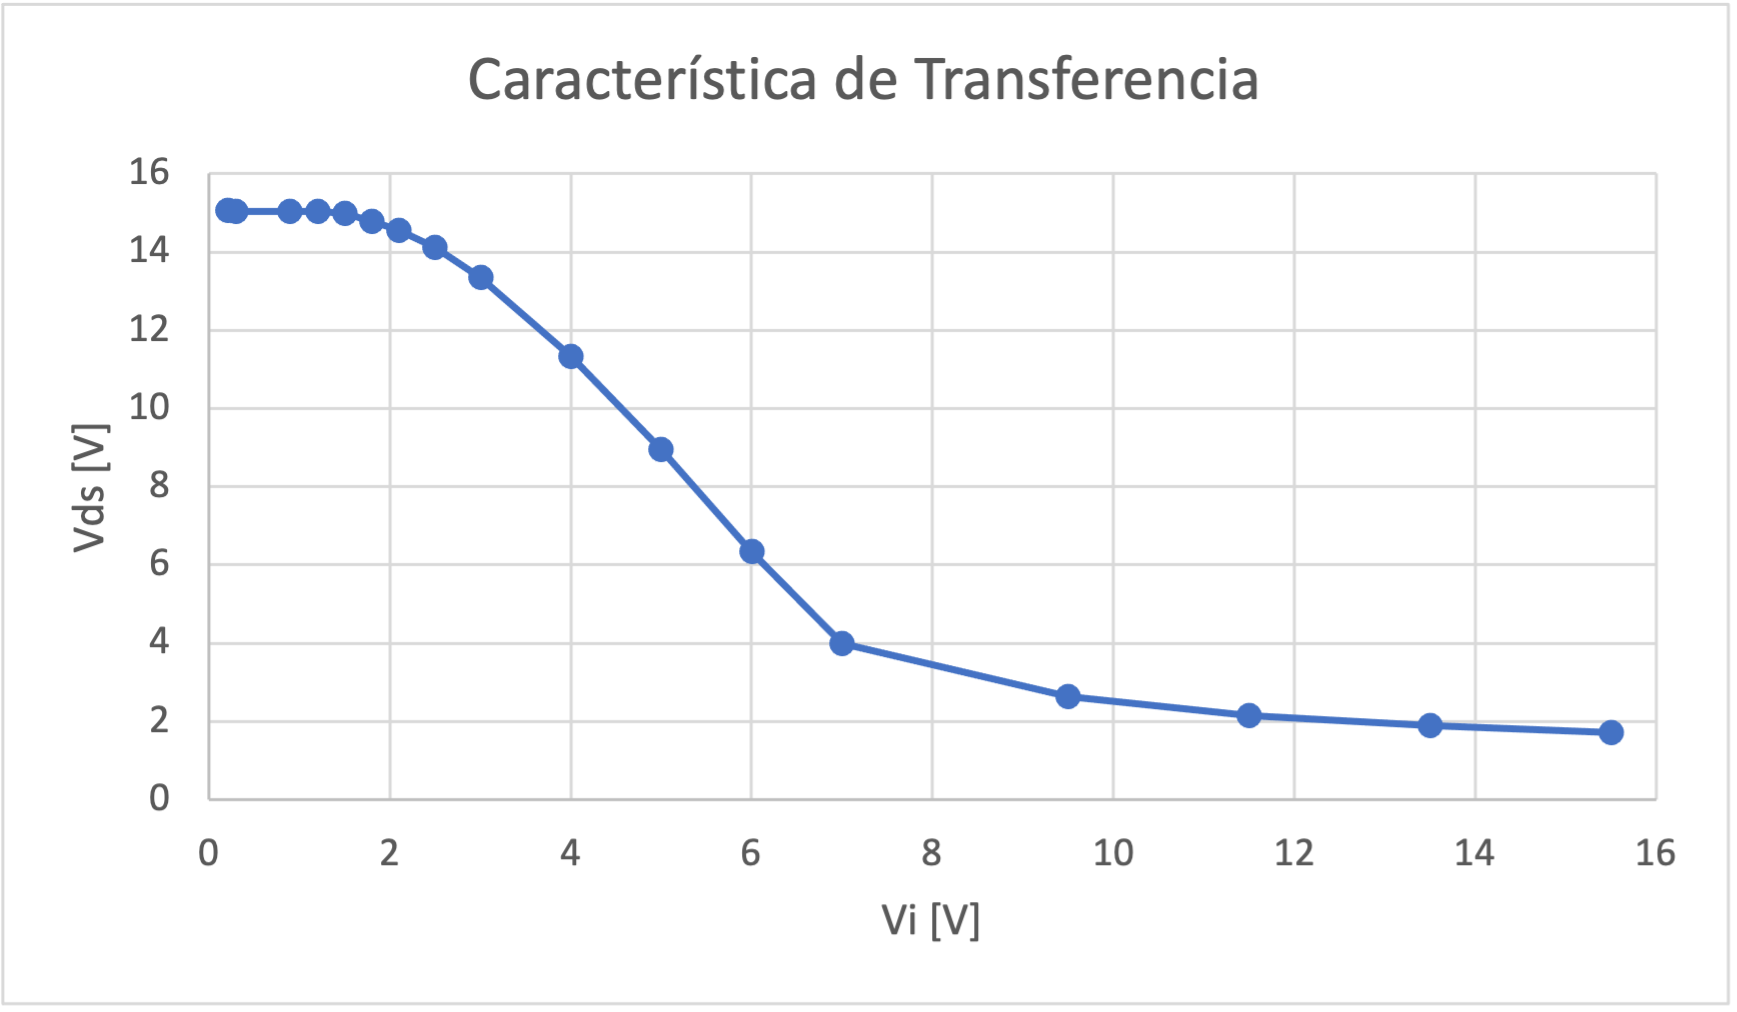
\includegraphics[width=13cm]{Imágenes 05/CarTrans_Exp.png}
    \caption{Característica de Transferencia del circuito \ref{fig:Circuito_CarTrans} tomando como salida $V_{DS}$}
    \label{fig:CarTrans_Exp}
\end{figure}

\newpage
\subsection{Curva I-V de un NMOSFET en saturación}
Se ha montado el circuito de la figura \ref{fig:Circuito_I-V}, donde el valor de $R_D$ es el mismo que en el circuito anterior.
\begin{itemize}
    \item $R_D = 0.998\;k\Omega$
\end{itemize}

Posteriormente, se han medido diversas magnitudes conforme se variaba el valor de $V_i$, el potencial de entrada. Los datos obtenidos se muestran en la figura \ref{fig:Datos_I-V}, donde cada columna representa:
\begin{description}
    \item [Columna 1:] Potencial de entrada real ($V_i^{exp}$) [$V$]. Medido con el polímetro.
    \item [Columna 2:] Caída de potencial en entre la puerta y la fuente del transistor ($V_{GS}$) [$V$]. Medido con el polímetro. Este es igual a la caída de potencial entre el drenador y la fuente, al estar drenador y puerta cortocircuitados ($V_{GS}=V_{DS}$).
    \item [Columna 3:] Caída de potencial en la resistencia del drendor ($V_{RD}$) [$V$]. Medido con el polímetro.
    \item [Columna 4:] Intensidad que circula entre el drenador y la fuente [$A$].\\ Calculada como $I_D = \frac{V_{RD}}{R_D}$.
    \item [Columna 5:] Raíz cuadrada de la intensidad que circula entre el drenador y la fuente ($\sqrt{I_D}$).
\end{description}

\begin{figure}
    \centering
    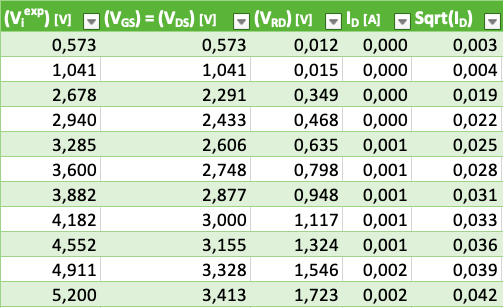
\includegraphics[width=8cm]{Imágenes 05/Tabla_Datos_CurvaI-V.png}
    \caption{Datos obtenidos en el circuito de la figura \ref{fig:Circuito_I-V}.}
    \label{fig:Datos_I-V}
\end{figure}

En la figura \ref{fig:CurvaI-V_Exp} se representa la relación entre $V_{GS}$ e $I_D$ en un transistor NMOSFET en saturación (circuito de la figura \ref{fig:Circuito_I-V}). Como se desea que el transistor esté en saturación, no se representan los valores para los que el transistor está en corte, es decir, el valor de $I_D$ sea despreciable.

\begin{figure}
    \centering
    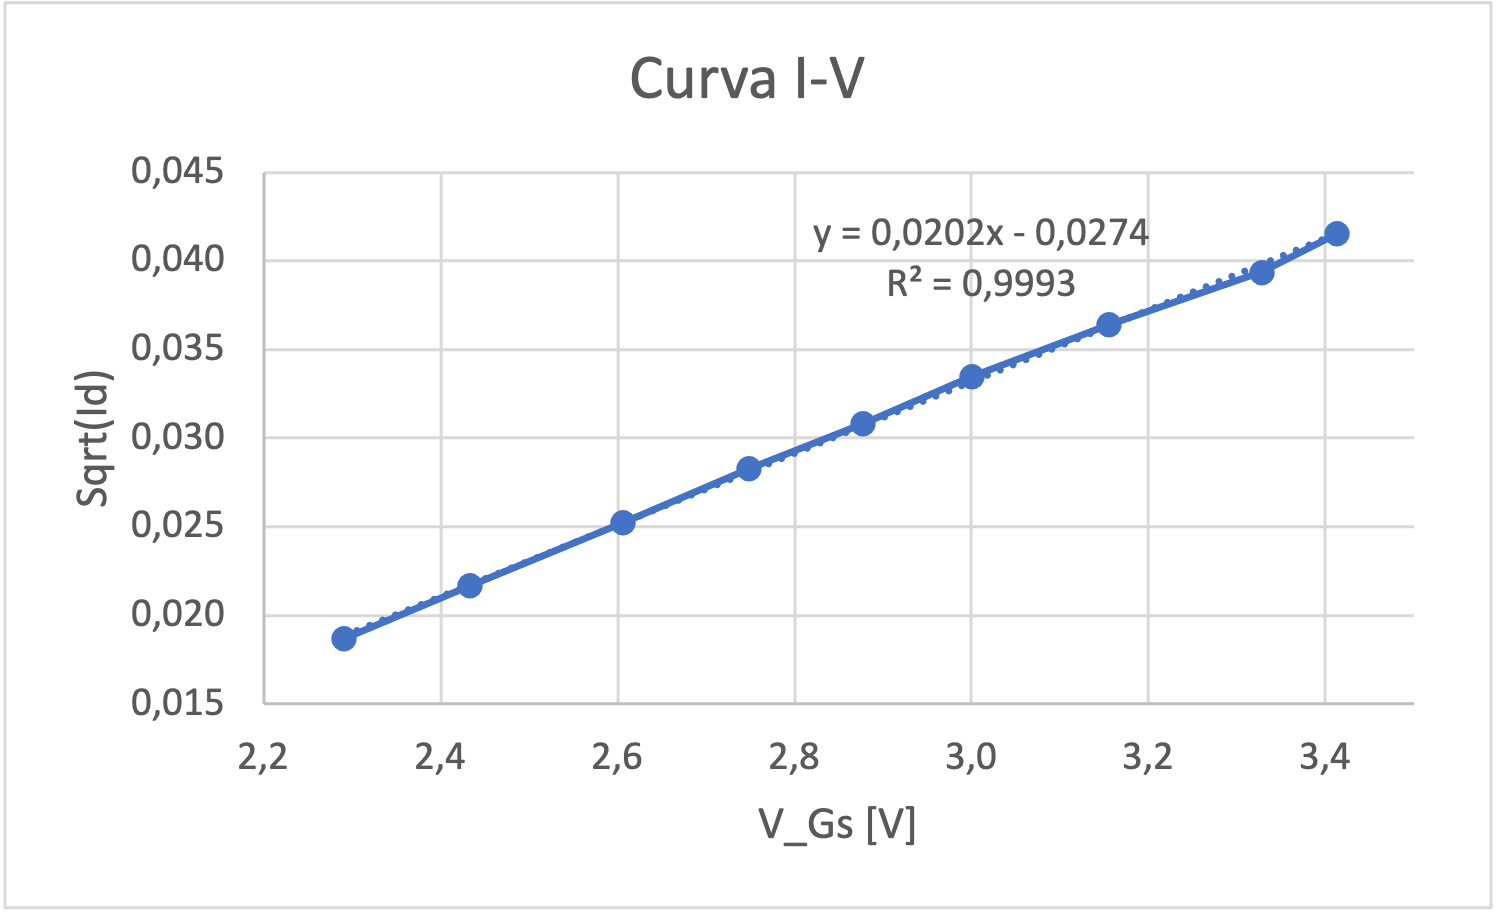
\includegraphics[width=11cm]{Imágenes 05/CurvaI-V_Exp.png}
    \caption{Característica de Transferencia del circuito \ref{fig:Circuito_I-V} tomando como salida $V_{DS}$.}
    \label{fig:CurvaI-V_Exp}
\end{figure}


\section{Discusión}

\subsection{Curva I-V de un NMOSFET en saturación}

En esta parte de la práctica, se ha representado la intensidad que circula por el transistor frente a el potencial de entrada $V_i=V_GS$. Tan solo se han representado aquellos valores para los que el transistor está en saturación, por lo que, teóricamente (ver Ec. \ref{Ec:Sat}):
\begin{equation}\begin{split}
    I_d = \frac{k}{2}(V_{GS}-V_T)^2 \Longrightarrow \sqrt{I_d} & = \sqrt{\frac{k}{2}}\;(V_{GS}-V_T)\\
     & = \sqrt{\frac{k}{2}}\;V_{GS} - \sqrt{\frac{k}{2}}\;V_T
\end{split}\end{equation}

Tras obtener la linea de tendencia lineal de la figura \ref{fig:CurvaI-V_Exp} con $R^2 = 0.993 \approx 1$ (muy fiable), vemos que:
\begin{equation}
    I_d \approx 0.0202 \;V_{GS} - 0.0274
\end{equation}

Por tanto,
\begin{equation}
\begin{split}
    & \sqrt{\frac{k}{2}} \approx 0.0202 \Longrightarrow k \approx 0.0202^2 \cdot 2 = 8.1608\cdot 10^-4 \; A/V\\
    & \sqrt{\frac{k}{2}} \; V_T \approx 0.0274 \Longrightarrow V_T \approx \frac{0.0274}{\sqrt{\frac{k}{2}}} = 1.35\;V
\end{split}
\end{equation}

Por tanto, los datos obtenidos experimentalmente para este diodo son:
\begin{itemize}
    \item $k \approx 8.1608\cdot 10^-4 \; A/V^2 $
    \item $V_T \approx 1.35\;V$
\end{itemize}

Estos resultados son razonables, ya que están en el orden de magnitud esperado. Además, en la figura \ref{fig:Datos_I-V} se aprecia cómo $I_G=0\;$, ya que, como predice la teoría, por la puerta del transistor la intensidad es siempre nula.


\subsection{Característica de transferencia}
Según el apartado anterior, $V_T = 1.35\;V$, valor para el cual el transistor pasa de estar en corte al estado de saturación.
El valor para el cual pasa de saturación a la región lineal es $V_i^*$, que tomando los datos del apartado anterior y la ecuación \ref{Ec:SatALin_CarTrans}, $V_i^*= 6.31\;V$.

Por tanto, en la figura \ref{fig:CarTrans_Teo} se representa la característica de transferencia teórica calculada en la ecuación \ref{Ec:CarTrans}, donde se han resaltado los puntos en los que el transistor cambia de estado. Como podemos ver, la gráfica experimental se asemeja considerablemente a lo que predice la teórica. Sí es verdad que no coincide exactamente, pero se debe a que al estar trabajando con una magnitud de orden tan pequeña, cualquier pequeño cambio destaca considerablemente.
\begin{figure}
    \centering
    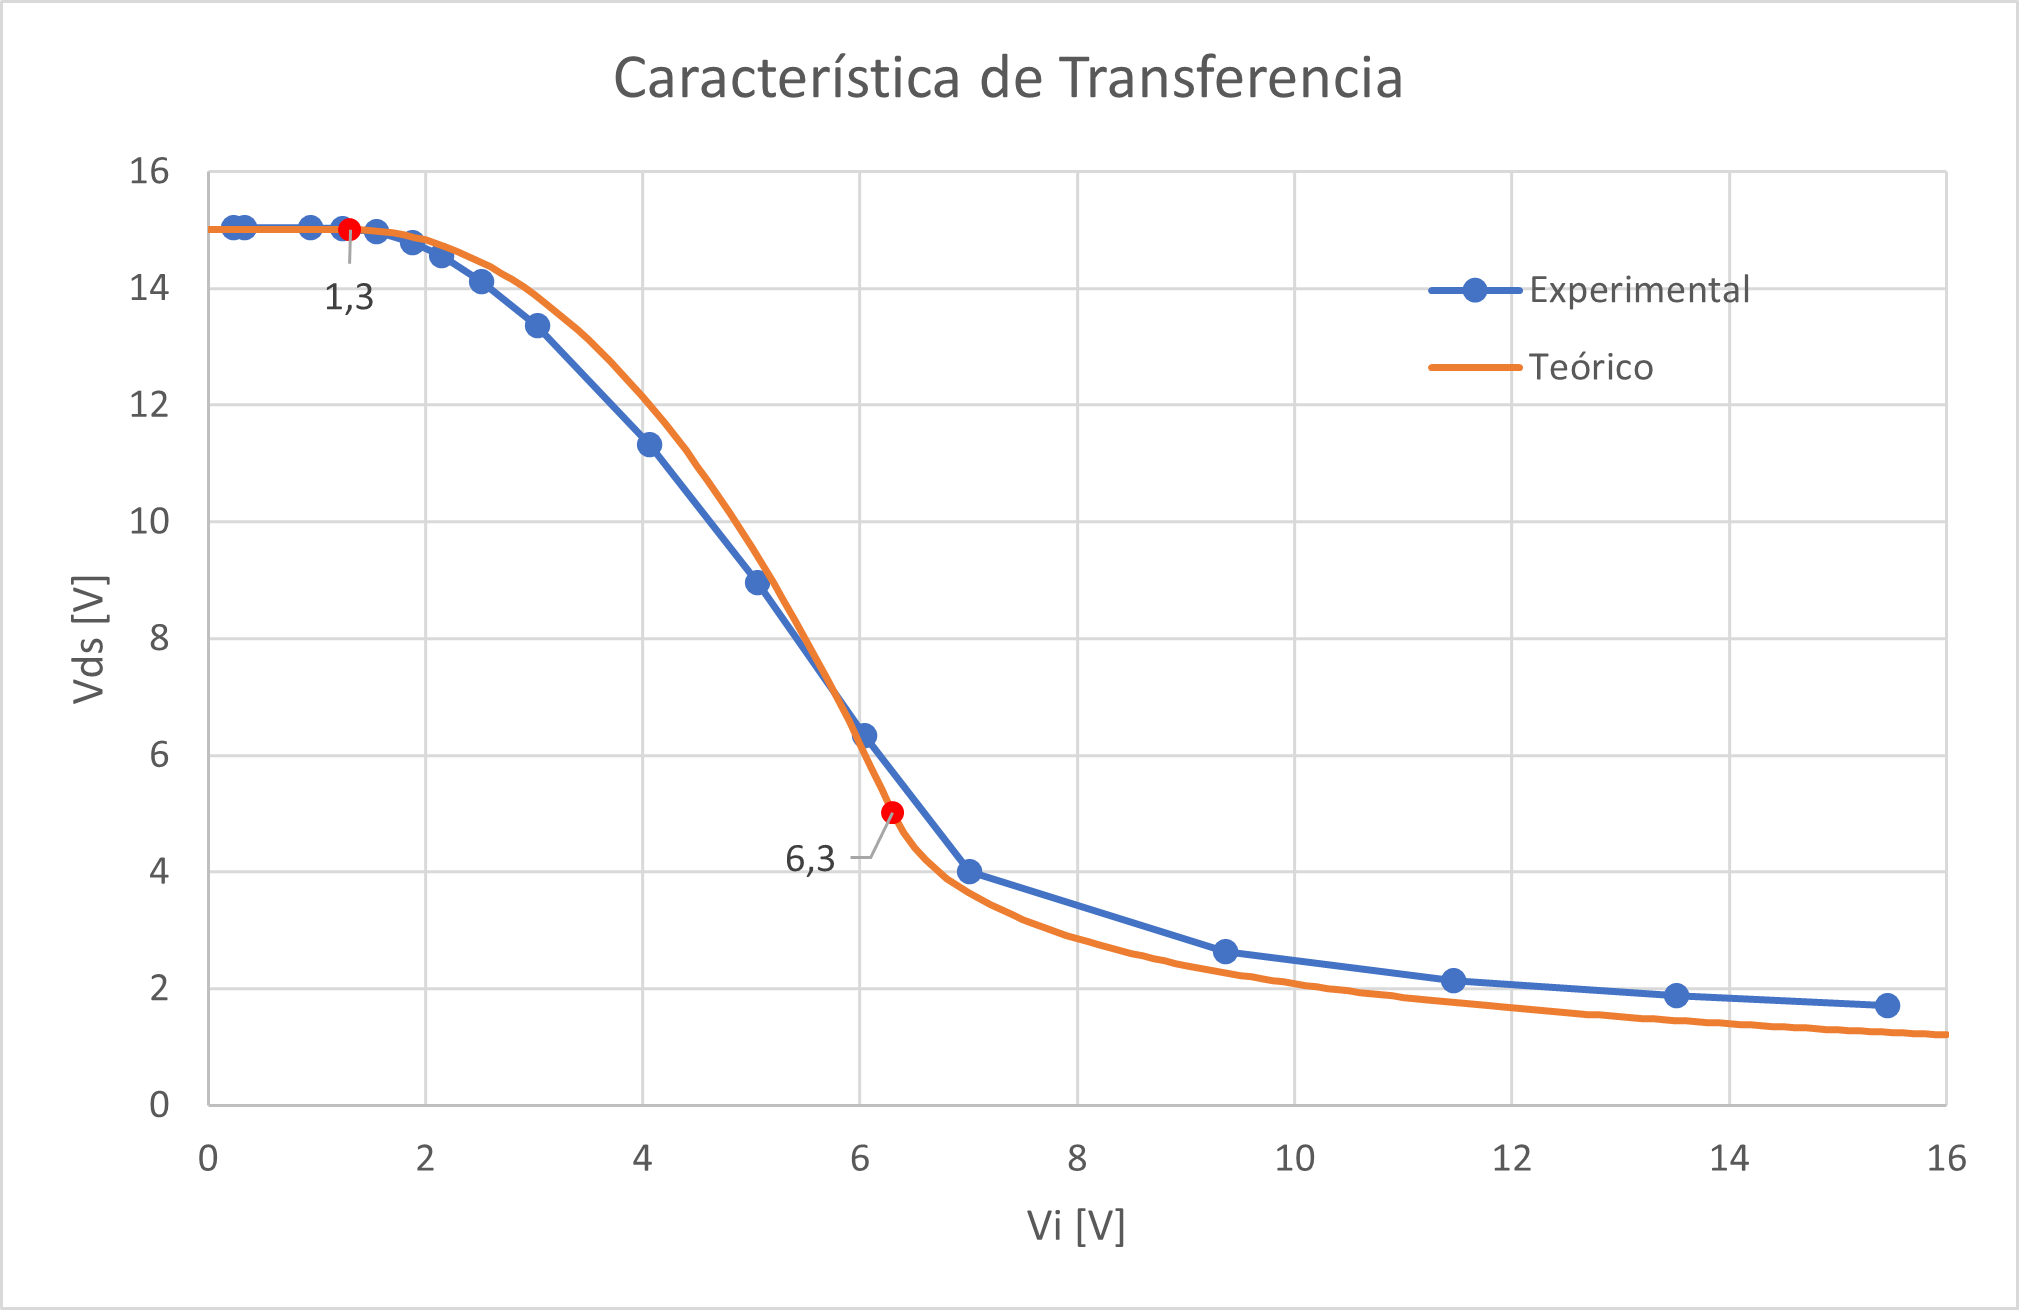
\includegraphics[width=12cm]{Imágenes 05/CarTrans_Teo.png}
    \caption{Característica de transferencia teórica del circuito \ref{fig:Circuito_CarTrans}.}
    \label{fig:CarTrans_Teo}
\end{figure}

% Comentario de los ajustes
\begin{comment}
Además, se ha realizado un ajuste lineal en el tramo en el que el transistor está en corte y un ajuste lineal en el tramo en el que está en saturación. Veamos cada uno por separado.

\begin{description}
    \item [Corte]
    \begin{equation}
        V_0 = -0.0144\;V_i + 15.05
    \end{equation}
    Este ajuste lineal tiene coef. de correlación $R^2 = 0.7203$, no muy cercano a $1$. No obstante, nos aporta datos orientativos.
    Cuando el transistor está en corte, la teoría afirma que $V_0 = V_{DD}$. Como $-0.0144 \approx 0$ y $15.05\approx 15 = V_{DD}$, los resultados experimentales en este tramo se ajustan fielmente a la realidad.

    \item [Saturación]
    \begin{equation}
        V_0 = -0.2503\;V_i^2 - 0.0672\;V_i + 15.794
    \end{equation}
    En este caso, este ajuste polinómico de grado 2 tiene coeficiente de correlación $R^2=0.9993\approx1$, por lo que es muy fiable.
    Para este estado, la teoría afirma que:
    \begin{equation}\begin{split}
        V_0 & = V_{DD} - \frac{kR_D}{2}\;(V_i-V_T)^2\\
        & = -\frac{kR_D}{2}\;V_i^2 + (kR_pV_T)V_i + V_{DD} -\frac{kR_D}{2}\;V_T^2
    \end{split}\end{equation}

    Por tanto,
    $$
        -\frac{kR_D}{2} = -0.2503\Longrightarrow k = 0.2503 \; \frac{2}{R_D} = 5 \cdot 10^{-4}\;A/V^2
    $$
    $$
        kR_pV_T = -0.0672\Longrightarrow
    $$
        
\end{description}
\end{comment}



\section{Conclusiones}
Las conclusiones extraídas de esta práctica de laboratorio son:
\begin{itemize}
    \item En primer lugar, el circuito con un transistor tipo N y una resistencia como carga en el drenador (circuito \ref{Ec:CarTrans}) se ha visto que se comporta como un inversor. Este es fundamental en la electrónica digital actual, ya que es la base para las puertas lógicas del álgebra booleana como son las NAND, NOR, XOR o muchas otras. Estas son muy relevantes en la informática actual y son la base de muchos procesadores, por lo que este componente es esencial.

    \item Además, se ha podido observar como los datos predichos con la teoría coinciden, una vez más, con lo que sucede experimentalmente. Esto supone una gran ayuda, ya que permite estudiar diversos circuitos más complejos de forma teórica basándonos en los conocimientos teóricos.

    \item Por último, se ha podido comprobar la característica del transistor como \emph{semiconductor}, ya que en función del potencial de entrada se ha podido observar que se puede encontrar en tres regiones de funcionamiento distintas, todas ellas con valores de intensidad distintos.
\end{itemize}